\subsection{Overview Page}
\label{sec:overview-page}

The Overview Page is the main dashboard of the automation platform and the first page users see after logging in. It acts as a central workspace where users can manage the different parts of the system without having to switch between multiple pages. It provides a standardized layout architecture combining navigation, workflow management, credential storage, and execution monitoring into a single, filtered, paginated interface.

\begin{figure}[H]
    \centering
    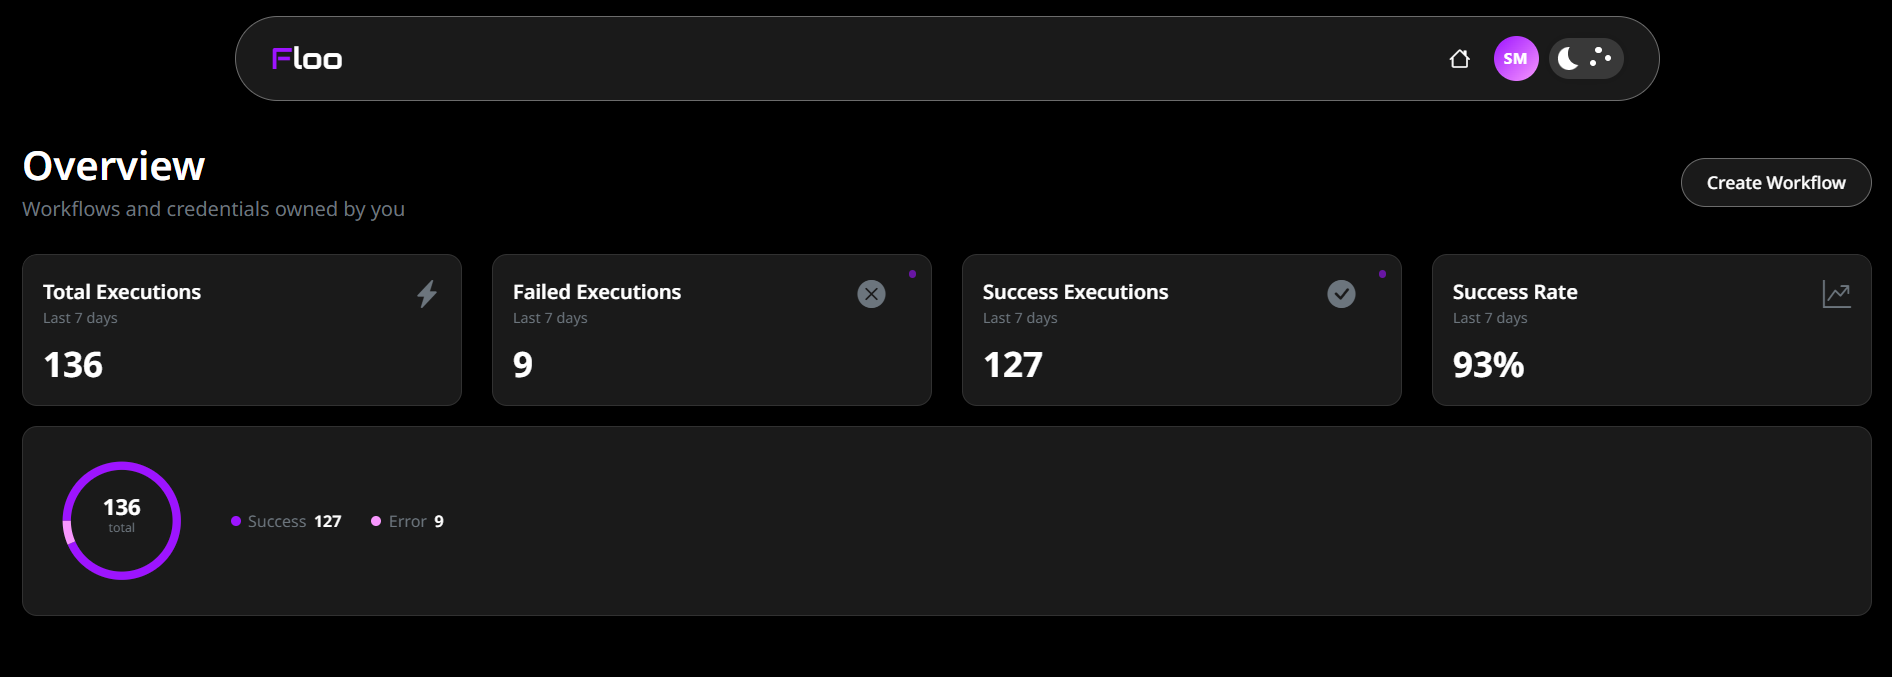
\includegraphics[width=\textwidth]{images/overview-page/overview-1.png}
    \caption{The Overview Page dashboard, showing the navigation bar, execution analysis cards, and execution status chart.}
    \label{fig:overview-nav}
\end{figure}

\subsubsection{OverviewNav Component}

\textbf{Purpose:} Acts as the persistent top navigation bar, exposing branding, theme controls, administrative shortcuts, and the user profile icon, while acting as a barrier that blocks unverified users from navigating to restricted pathways.

\vspace{0.2cm}
\noindent\textbf{Location:} \texttt{src/components/OverviewNav.jsx}

\vspace{0.2cm}
\noindent\textbf{Props:}
\begin{itemize}
    \item \texttt{firstName} (String): The user's first name, used to create the profile icon's initials.
    \item \texttt{lastName} (String): The user's last name, also used for the initials.
    \item \texttt{isVerified} (Boolean): Verification status flag that explicitly locks or unlocks general navigation pathways.
\end{itemize}

\vspace{0.2cm}
\noindent\textbf{Components Used:}
\begin{itemize}
    \item \texttt{NavIconBtn} --- A helper component that acts as either a clickable button or a page link, blocking the action when the user is not verified.
    \item \texttt{Avatar} --- A styled link component pointing to \texttt{/user-profile} that safely extracts, merges, and displays the uppercase first letters of the user's first and last names.
\end{itemize}

\vspace{0.2cm}
\noindent\textbf{Notes:}
\begin{itemize}
    \item Checks the user's account details and, if logged in as an admin, automatically reveals an extra lock icon (\texttt{bi-shield-lock}) that links to the admin user management screen.
    \item Holds the theme toggle button (\texttt{<ModeSwitch/>}) on the right side so users can switch between light and dark modes whenever they want.
    \item Uses a modern, semi-transparent effect that blurs the background slightly.
    \item On smaller screens, the layout shrinks automatically: padding is reduced, icon gaps tighten, the logo scales down, and the profile avatar shrinks so everything fits without clutter.
\end{itemize}


\subsubsection{CreateWorkflow Component}

\textbf{Purpose:} Handles creation of a brand-new automation project through a centered modal window containing a structured input form, safely processing project data and sending it to the server without refreshing the page.

\vspace{0.2cm}
\noindent\textbf{Location:} \texttt{src/pages/Overview/components/CreateWorkflow.jsx}

\vspace{0.2cm}
\noindent\textbf{Props:}
\begin{itemize}
    \item \texttt{onWorkflowCreated} (Function): A callback that fires right after the server successfully builds the workflow, passing the newly created workflow data upward so the dashboard can instantly update or redirect the user.
    \item \texttt{onClose} (Function): Dismisses and hides the popup modal when a user clicks ``Cancel,'' hits the top-right close icon, or clicks outside the window.
\end{itemize}

\vspace{0.2cm}
\noindent\textbf{Components Used:}
\begin{itemize}
    \item \texttt{WorkflowForm} --- Renders the input fields, textareas, and select menus inside the popup body, keeping the layout logic separated for readability.
\end{itemize}

\vspace{0.2cm}
\noindent\textbf{Notes:}
\begin{itemize}
    \item The dashboard ``Create Workflow'' button is disabled if the system is actively fetching background data or if the user has not verified their email.
    \item The form starts with reasonable defaults: an empty name field, a blank optional description, the workflow type set to ``Personal,'' and a baseline version number of 1.
    \item On submission, the handler trims whitespace from the optional description; if left blank, the field is omitted entirely from the API payload rather than sending blank text.
    \item Communicates directly with \texttt{WorkflowService.createWorkflow}. Errors are caught and displayed in a red alert box above the form fields; on success, the new workflow data is saved and the window closes immediately.
    \item While the API call runs, \texttt{isSubmitting} is set to true, disabling both the ``Cancel'' and ``Create Workflow'' buttons and replacing the submit text with a spinning loading wheel to prevent accidental double submissions.
\end{itemize}

\begin{figure}[h!]
    \centering
    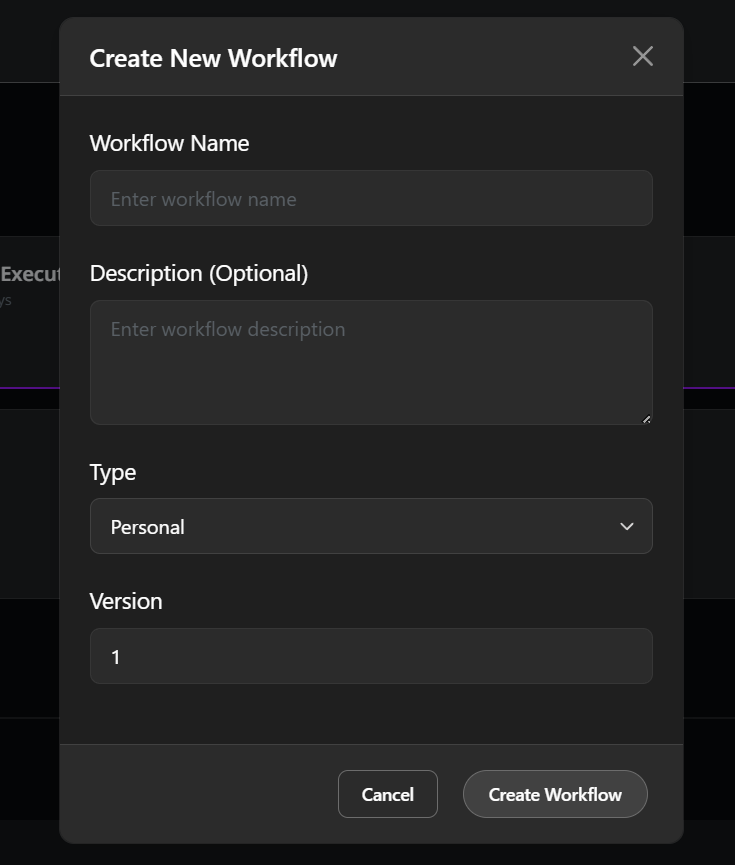
\includegraphics[width=0.7\textwidth]{images/overview-page/create-workflow-form.png}
    \caption{The Create Workflow modal, prompting for the workflow name, description, type, and version.}
    \label{fig:create-workflow-modal}
\end{figure}


\subsubsection{MetricsSection Component}

\textbf{Purpose:} Displays a high-level summary of workflow execution analytics collected over the previous seven days, combining key execution metrics with a visual execution distribution chart so users can evaluate workflow health directly from the dashboard.

\vspace{0.2cm}
\noindent\textbf{Location:} \texttt{components/MetricsSection.jsx}

\vspace{0.2cm}
\noindent\textbf{Props:}
\begin{itemize}
    \item \texttt{setAuth} (Function): Supplies authenticated requests with refreshed authorization information while retrieving execution analytics.
    \item \texttt{onMetricClick} (Function): Callback executed when users select an interactive metric card to filter the Executions tab according to the selected execution status.
    \item \texttt{onAnalyticsLoaded} (Function): Returns the retrieved analytics object to the parent Overview component after a successful fetch operation.
\end{itemize}

\vspace{0.2cm}
\noindent\textbf{Notes:}
\begin{itemize}
    \item Immediately after mounting, invokes \texttt{ExecutionService.getAnalytics()} requesting execution statistics for the previous seven days, displaying loading indicators until the data becomes available.
\end{itemize}

\begin{center}
\begin{minipage}{0.6\textwidth}
\begin{lstlisting}
const data = await ExecutionService.getAnalytics(
  { days: 7 },
  setAuth
);
\end{lstlisting}
\end{minipage}
\end{center}

\begin{itemize}
    \item Relies on a \texttt{METRICS\_CONFIG} configuration array rather than hardcoding each card; each object defines the title, subtitle, icon, formatting function, and applicable execution statuses, simplifying the addition of new metrics.
\end{itemize}

\begin{center}
\begin{minipage}{0.6\textwidth}
\begin{lstlisting}
const METRICS_CONFIG = [
  {
    key: "failedExecutions",
    title: "Failed Executions",
    filterStatus: ["ERROR", "FAILED", "CRASHED"],
    ...
  }
];
\end{lstlisting}
\end{minipage}
\end{center}

\begin{itemize}
    \item Each \texttt{MetricCard} appears using a staggered entrance animation, and numeric values animate through an incremental counter until reaching the final value.
    \item The Failed Executions and Success Executions cards act as interactive controls: selecting either invokes \texttt{onMetricClick}, switching the Overview page to the Executions tab while applying the corresponding status filter.
\end{itemize}

\begin{center}
\begin{minipage}{0.6\textwidth}
\begin{lstlisting}
onClick={() =>
  isClickable && onMetricClick(filterStatus)
}
\end{lstlisting}
\end{minipage}
\end{center}

\begin{itemize}
    \item After analytics are retrieved, renders the \texttt{<ExecutionChart />} component to present a graphical breakdown of execution states.
\end{itemize}

\begin{center}
\begin{minipage}{0.6\textwidth}
\begin{lstlisting}
{!isLoading && analytics && (
  <ExecutionChart analytics={analytics} />
)}
\end{lstlisting}
\end{minipage}
\end{center}

\begin{itemize}
    \item While analytics are being fetched, each metric card displays a loading spinner in place of its numeric value; unavailable metrics show placeholder values to preserve a consistent layout.
\end{itemize}


\subsubsection{ExecutionChart Component}

\textbf{Purpose:} Provides a visual summary of workflow execution results by displaying a donut chart representing the distribution of execution statuses over the selected analytics period.

\vspace{0.2cm}
\noindent\textbf{Location:} \texttt{components/ExecutionChart.jsx}

\vspace{0.2cm}
\noindent\textbf{Props:}
\begin{itemize}
    \item \texttt{analytics} (Object): Analytics object containing the execution status breakdown returned by the analytics service.
\end{itemize}

\vspace{0.2cm}
\noindent\textbf{Notes:}
\begin{itemize}
    \item Extracts execution counts from the \texttt{statusBreakdown} object and computes the total number of executions; returns \texttt{null} if no execution data exists, preventing unnecessary rendering.
    \item Builds an internal collection of execution categories, assigning each status a predefined color and label; statuses with zero executions are automatically removed from the visualization.
    \item Generates the donut chart using SVG \texttt{<circle>} elements, with \texttt{strokeDasharray} and \texttt{strokeDashoffset} dynamically computed to position every segment consecutively around the circle based on its proportion of the total.
    \item Displays the total number of executions in the center of the donut chart for an immediate numerical summary.
    \item On smaller screens, rearranges the chart and legend vertically to preserve readability while maintaining consistent spacing across devices.
\end{itemize}


\subsubsection{WorkflowList Component}

\textbf{Purpose:} Acts as the central control hub for managing a user's automated pipelines, handling client-side filtering, sequential page distribution, card selection redirects, and item deletion cleanup syncs. Rendered while the Workflows tab is active within the dashboard's tabbed content area (\texttt{content-tabs}).

\begin{figure}[H]
    \centering
    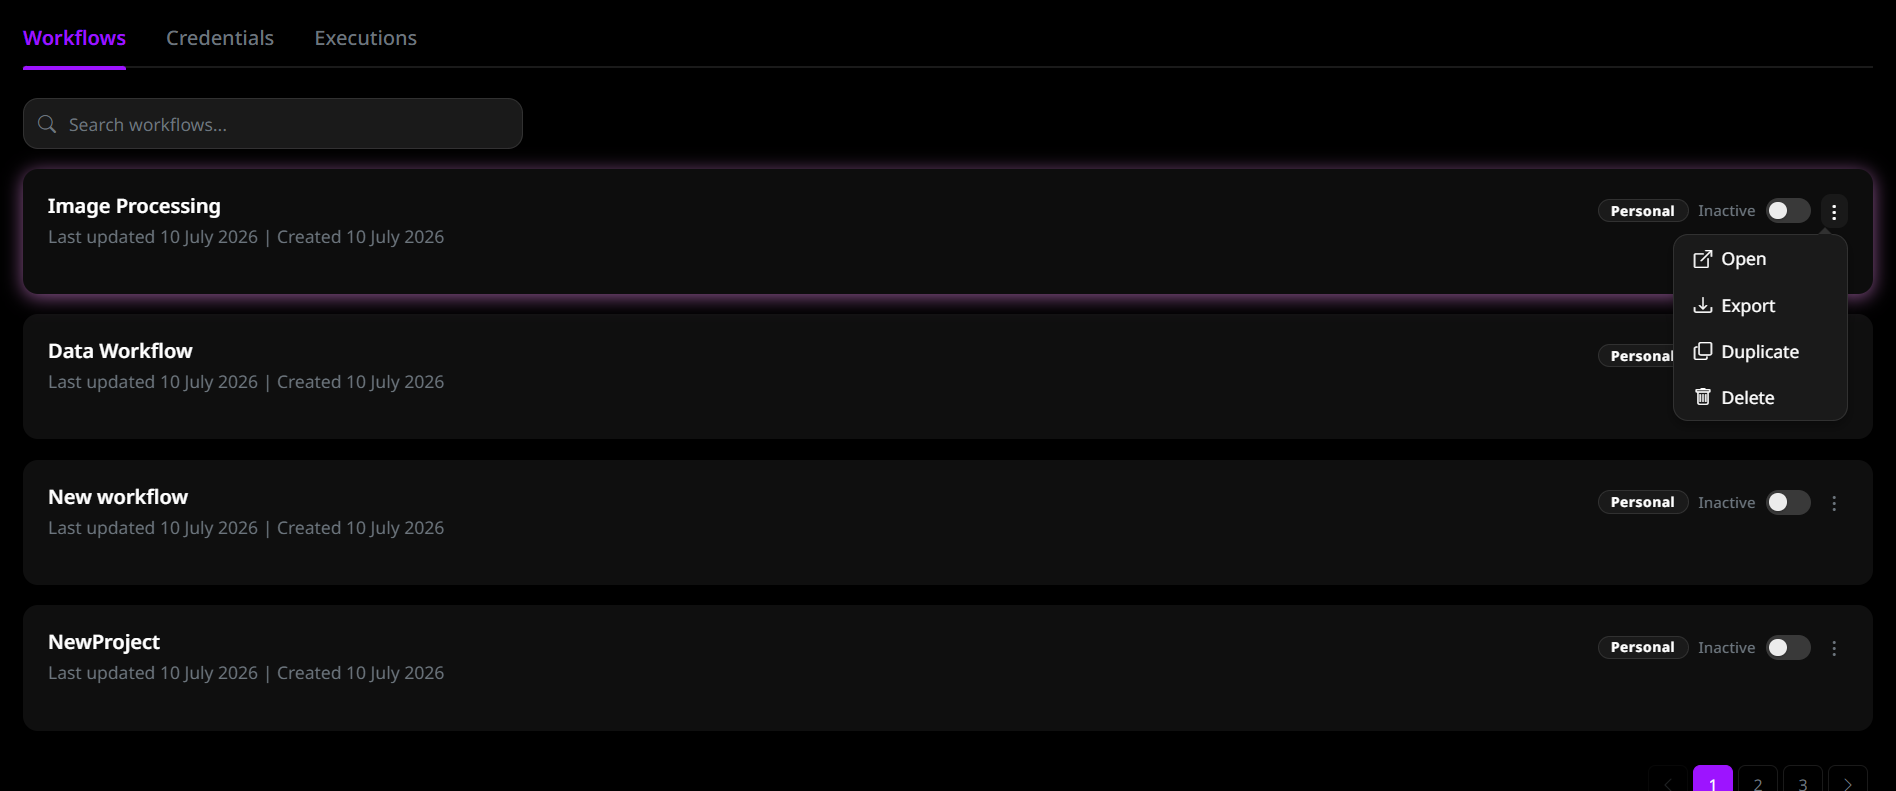
\includegraphics[width=\textwidth]{images/overview-page/workflows-tab.png}
    \caption{The Workflows tab, showing the workflow list with the action menu open for a selected workflow.}
    \label{fig:workflows-tab}
\end{figure}

\vspace{0.2cm}
\noindent\textbf{Location:} \texttt{src/components/WorkflowList.jsx} (paired with \texttt{src/components/styles/WorkflowList.css})

\vspace{0.2cm}
\noindent\textbf{Props:}
\begin{itemize}
    \item \texttt{workflows} (Array): The raw list of workflow objects fetched from the database.
    \item \texttt{onWorkflowDeleted} (Function): Callback fired to notify parent components when a workflow is successfully removed.
    \item \texttt{refetch} (Function): Triggers a global data reload to refresh the dashboard state.
\end{itemize}

\vspace{0.2cm}
\noindent\textbf{Notes:}
\begin{itemize}
    \item Uses a \texttt{useEffect} hook to watch the \texttt{initialWorkflows} prop; whenever parent data changes, updates the local \texttt{workflows} state and resets the page view back to 1.
    \item Filters the array case-insensitively against the search text, forcing both values to lowercase to guarantee accurate matching.
    \item Slices the filtered array into segments using a fixed limit of items per page (\texttt{PAGE\_SIZE = 4}); changing or clearing the search text snaps the pagination tracker back to page 1 to prevent out-of-bounds rendering.
    \item Tracks the currently open action menu by ID (\texttt{openMenuId}); when a card's dropdown opens, assigns a specialized \texttt{.dropdown-open} class to that item container.
\end{itemize}

\vspace{0.2cm}
\noindent\textbf{WorkflowActions Sub-Component}

\vspace{0.2cm}
\noindent\textbf{Purpose:} Provides an action menu for each workflow, allowing users to open, export, duplicate, or delete workflows while coordinating backend operations and synchronizing the user interface.

\vspace{0.2cm}
\noindent\textbf{Location:} Declared inline or as a sub-module alongside \texttt{WorkflowList.jsx}.

\vspace{0.2cm}
\noindent\textbf{Props:}
\begin{itemize}
    \item \texttt{workflow} (Object): Contains the complete metadata of the selected workflow.
    \item \texttt{setAuth} (Function): Supplies authenticated requests with refreshed authorization information.
    \item \texttt{onDelete} (Function): Removes the deleted workflow from the parent component after successful deletion.
    \item \texttt{onOpen} (Function): Opens the selected workflow in the workflow editor.
    \item \texttt{refetch} (Function): Reloads the workflow collection after operations that modify the dataset.
    \item \texttt{isOpen} (Boolean): Indicates whether the action dropdown menu is currently visible.
    \item \texttt{onToggle} (Function): Controls the visibility state of the dropdown menu.
\end{itemize}

\vspace{0.2cm}
\noindent\textbf{Notes:}
\begin{itemize}
    \item Every action inside the dropdown calls \texttt{e.stopPropagation()} to prevent the parent workflow card's click handler from opening the workflow editor while interacting with menu options.
    \item Embeds the \texttt{<WorkflowToggle/>} component, allowing users to activate or deactivate a workflow directly. The toggle performs an optimistic UI update, then invokes \texttt{WorkflowService.executeWorkflow()} or \texttt{WorkflowService.stopWorkflow()} accordingly, rolling back the toggle state automatically if the server operation fails.
\end{itemize}

\begin{center}
\begin{minipage}{0.6\textwidth}
\begin{lstlisting}
<WorkflowToggle
  isActive={workflow.deployed}
  workflowId={workflow.id}
  setAuth={setAuth}
  onToggle={refetch}
/>
\end{lstlisting}
\end{minipage}
\end{center}

\begin{itemize}
    \item Selecting Export invokes the asynchronous \texttt{exportWorkflow()} helper, temporarily disabling the export option to prevent duplicate requests. On success, a sanitized filename is generated via \texttt{slugifyFilename()} and the exported workflow is displayed inside the \texttt{JsonPopup} modal.
    \item Stores the exported workflow inside the \texttt{exportModal} state object, controlling the visibility and content of \texttt{<JsonPopup />}, which allows users to inspect, download, or copy the exported workflow.
\end{itemize}

\begin{center}
\begin{minipage}{0.6\textwidth}
\begin{lstlisting}
<JsonPopup
  show={exportModal.show}
  onClose={handleCloseExportModal}
  data={exportModal.data}
  filename={exportModal.filename}
  title={workflow.name}
/>
\end{lstlisting}
\end{minipage}
\end{center}

\begin{itemize}
    \item Duplication first exports the selected workflow via the existing export endpoint, then submits the returned definition to the backend import endpoint (\texttt{POST /api/project/import}) together with the current project identifier, merging metadata such as name, type, and description before sending. On success, \texttt{refetch()} retrieves the updated workflow list.
    \item Selecting Delete sends a \texttt{DELETE} request to the backend; on success, notifies the parent through \texttt{onDelete()} so the removed workflow disappears without a full page refresh.
    \item Manages dropdown visibility through the \texttt{isOpen} and \texttt{onToggle} props, registering a document-level click listener while the dropdown is open so clicking outside automatically closes it.
\end{itemize}

\begin{figure}[h!]
    \centering
    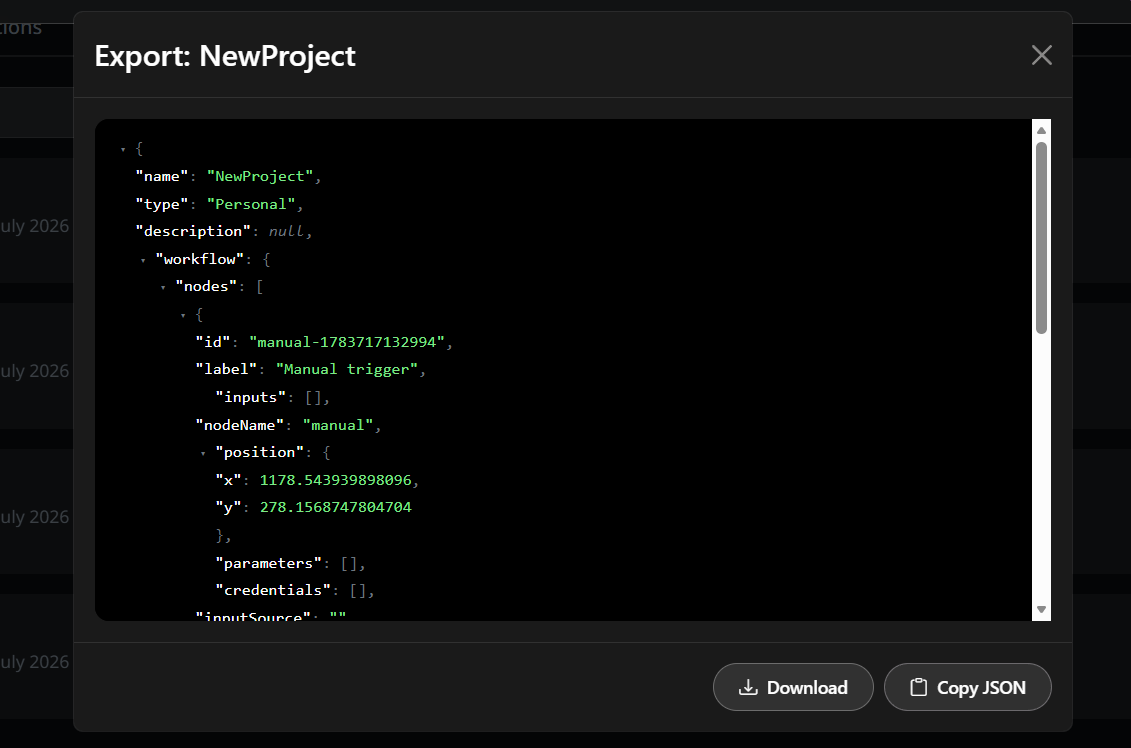
\includegraphics[width=0.95\textwidth]{images/overview-page/json-popup.png}
    \caption{The JSON export popup, showing the workflow structure with download and copy options.}
    \label{fig:json-export-popup}
\end{figure}

\vspace{0.2cm}
\noindent\textbf{NoWorkflows Sub-Component}

\vspace{0.2cm}
\noindent\textbf{Purpose:} Provides a clean placeholder screen when a user's directory contains no automation blueprints, offering a clear onboarding flow toward creating their first workflow.

\vspace{0.2cm}
\noindent\textbf{Location:} \texttt{src/components/NoWorkflows.jsx} (paired with \texttt{src/components/styles/NoWorkflows.css})

\vspace{0.2cm}
\noindent\textbf{Props:}
\begin{itemize}
    \item \texttt{onAddWorkflow} (Function): Callback action triggered when a user clicks the visual creation card.
\end{itemize}

\vspace{0.2cm}
\noindent\textbf{Notes:}
\begin{itemize}
    \item Implements a direct click capture on the central card container; clicking anywhere on the card fires the \texttt{onAddWorkflow} callback to open creation wizards or modal forms.
\end{itemize}


\subsubsection{CredentialsList Component}

\begin{figure}[h!]
    \centering
    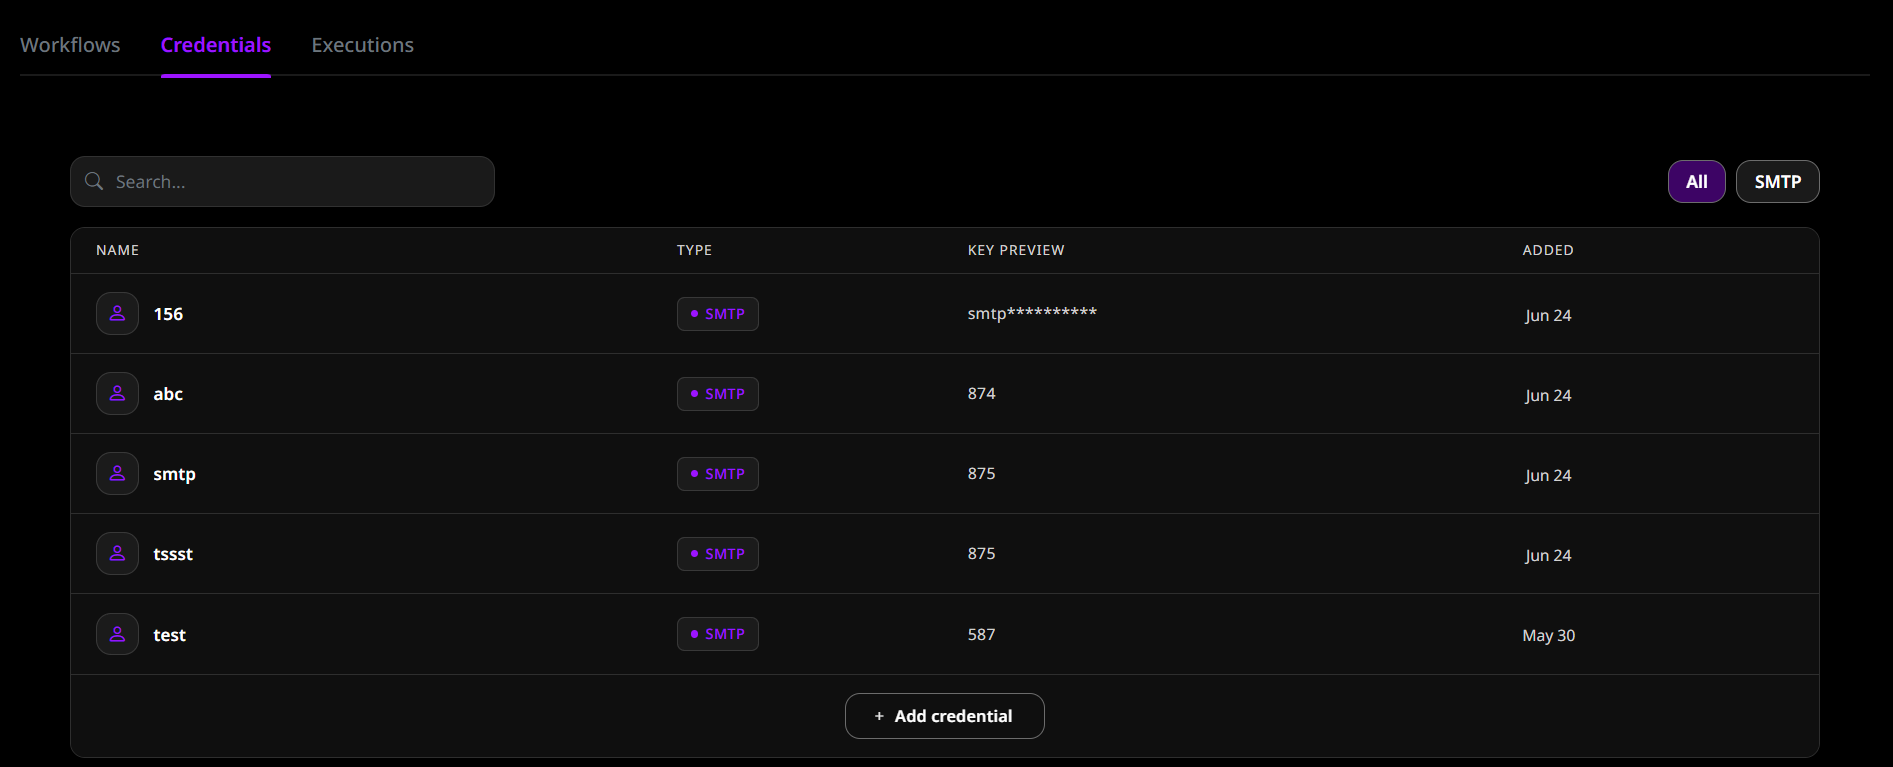
\includegraphics[width=\textwidth]{images/overview-page/credentials-tab.png}
    \caption{The Credentials tab, showing the searchable, filterable credentials table with masked key previews.}
    \label{fig:credentials-tab}
\end{figure}

\textbf{Purpose:} Serves as the main interface for managing the user's saved credentials, allowing users to search and filter credentials by type, view key information in a structured table, and create, edit, or delete credentials without leaving the dashboard.

\vspace{0.2cm}
\noindent\textbf{Location:} \texttt{src/components/CredentialsList.jsx}

\vspace{0.2cm}
\noindent\textbf{Props:}
\begin{itemize}
    \item \texttt{setAuth} (Function): Updates the user's authentication state if a request requires refreshing login credentials or handling authorization errors.
\end{itemize}

\vspace{0.2cm}
\noindent\textbf{Components Used:}
\begin{itemize}
    \item \texttt{AddCredential} --- A drawer-based form used to create new credentials or edit existing ones. Documented in full in Subsection~\ref{sec:addcredential}.
\end{itemize}

\vspace{0.2cm}
\noindent\textbf{Notes:}
\begin{itemize}
    \item Retrieves all saved credentials through the \texttt{useCredentials} hook, displaying a loading indicator during the request and an error message with a retry button on failure.
    \item Allows users to search credentials by name or type using the search box; filter buttons are generated automatically from the available credential types.
    \item Clicking Add Credential opens the \texttt{AddCredential} drawer empty; editing passes the selected credential to the same drawer, which automatically switches to edit mode.
    \item Masks credential information before rendering it in the table --- email addresses and long keys are partially hidden to protect sensitive data while still allowing identification.
    \item Action buttons remain hidden until the user hovers over a credential row, from where they can edit or delete the credential; deletions immediately update the displayed list.
    \item On smaller devices, less important columns such as key preview and added date are hidden, while the search bar and filter buttons rearrange to maintain a clean interface.
\end{itemize}


\subsubsection{AddCredential Component}
\label{sec:addcredential}

\textbf{Purpose:} Provides a drawer-based interface for creating new credentials and updating existing ones, dynamically generating input fields based on the selected credential type, validating user input, and securely submitting credential information without leaving the dashboard.

\begin{figure}[h!]
    \centering
    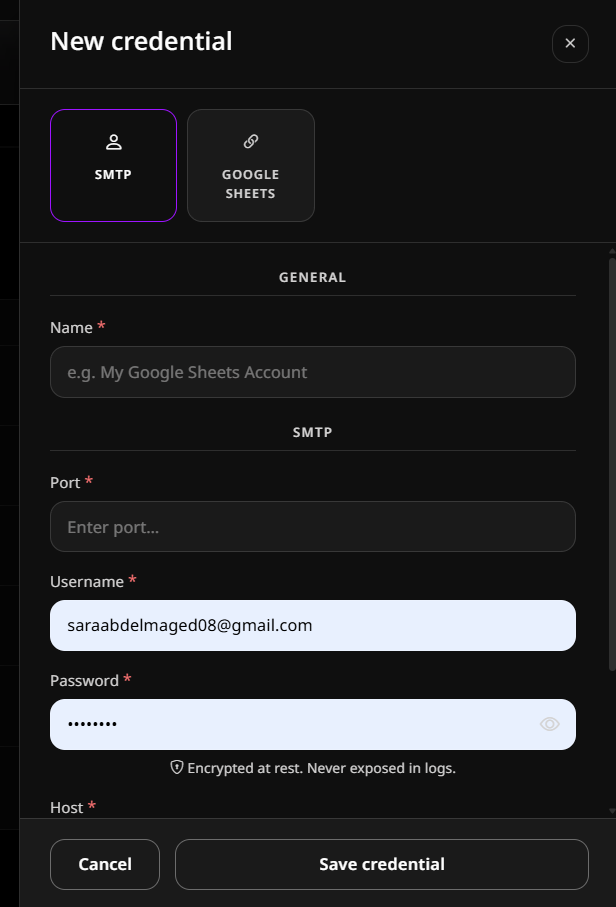
\includegraphics[width=0.5\textwidth]{images/overview-page/add-credential.png}
    \caption{The Add Credential drawer}
    \label{fig:add-credential-drawer}
\end{figure}

\vspace{0.2cm}
\noindent\textbf{Location:} \texttt{src/components/AddCredential.jsx}

\vspace{0.2cm}
\noindent\textbf{Props:}
\begin{itemize}
    \item \texttt{open} (Boolean): Controls whether the credential drawer is visible.
    \item \texttt{onClose} (Function): Closes the drawer and resets its state.
    \item \texttt{onSave} (Function): Receives the credential data and handles creating or updating the credential.
    \item \texttt{setAuth} (Function): Updates the user's authentication state if authorization needs to be refreshed.
    \item \texttt{editCredential} (Object): The credential being edited. If no value is provided, the component opens in create mode.
\end{itemize}

\vspace{0.2cm}
\noindent\textbf{Notes:}
\begin{itemize}
    \item When \texttt{editCredential} is passed, the form is automatically populated with its current values, the title changes to Edit Credential, and the credential type is locked to prevent accidental changes.
    \item On open, loads the available credential types as selectable tabs; selecting a type retrieves its parameter definitions and automatically generates the required input fields.
    \item Builds input fields from the credential type definition returned by the server rather than using a fixed form, allowing different credential types to reuse the same interface.
    \item Validates the credential name and all required parameters before saving; fields with missing values are highlighted and validation messages are displayed without sending an invalid request.
    \item Parameters marked as sensitive are rendered as password fields with a visibility toggle, remaining hidden by default and clearly indicated as securely stored.
    \item After successful validation, prepares the credential payload and passes it to the parent through \texttt{onSave}; action buttons are disabled during submission to prevent duplicate requests.
    \item Displays loading indicators while credential types or parameter definitions are being retrieved; errors preserve the entered information so the user can retry.
    \item Uses animated transitions when opening and closing the drawer; closing clears the form, resets the selected credential type, and removes any temporary validation or error state.
\end{itemize}


\subsubsection{ExecutionsList Component}

\textbf{Purpose:} Displays the execution history of the user's workflows in a structured table, allowing users to monitor workflow runs, view execution status, apply status-based filters, and navigate through execution records using pagination.

\begin{figure}[H]
    \centering
    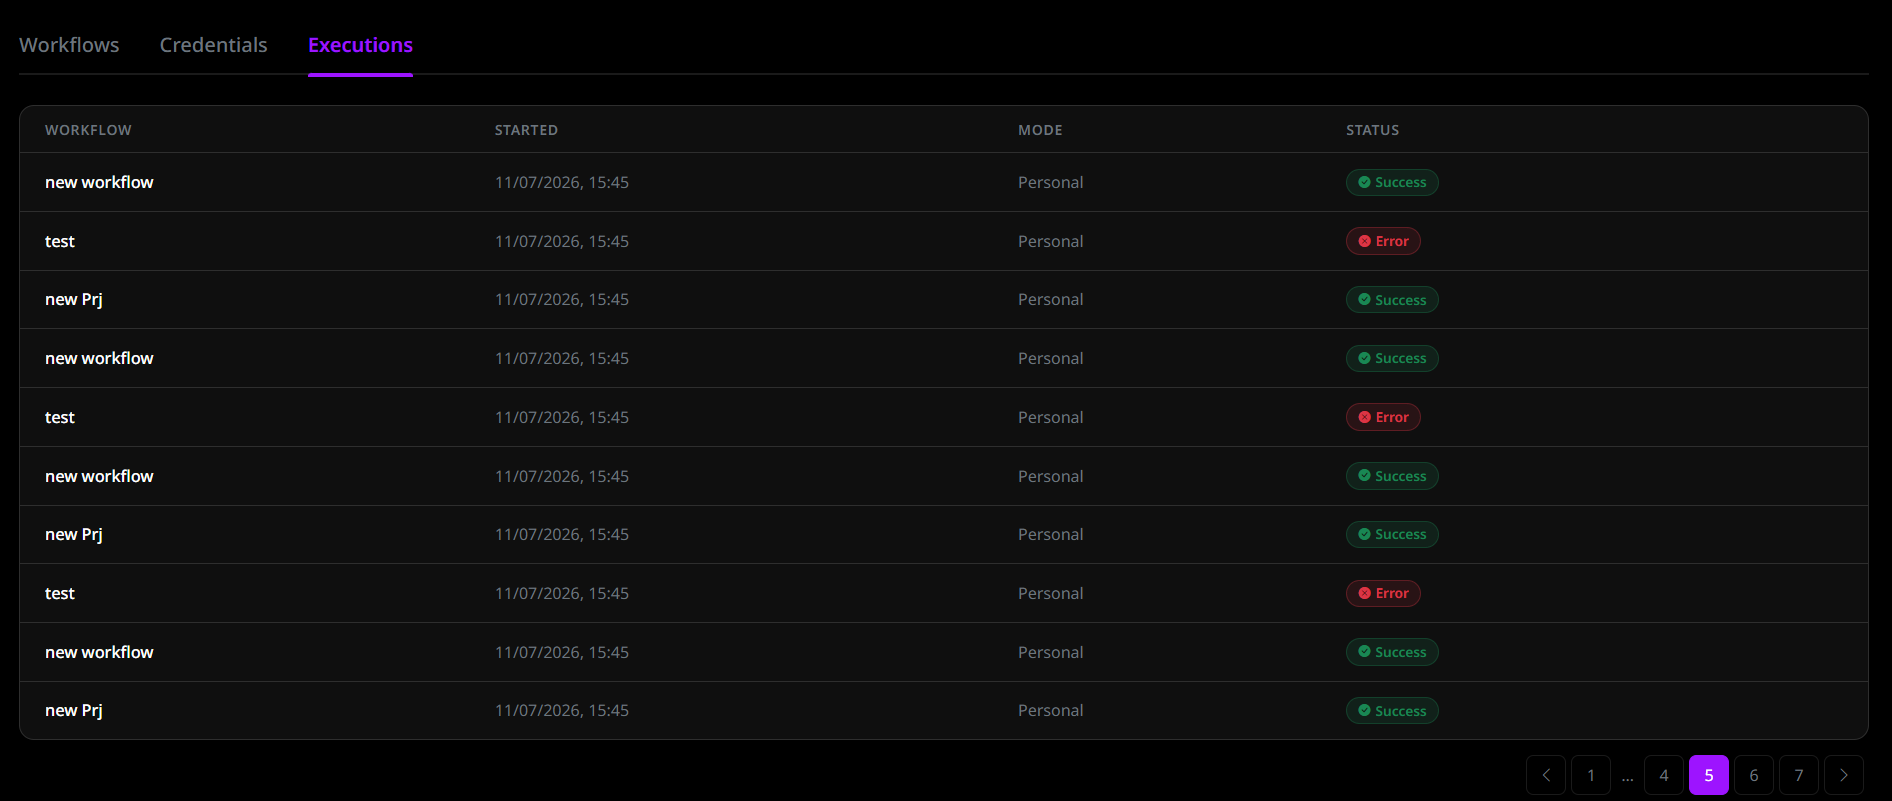
\includegraphics[width=\textwidth]{images/overview-page/executions-tab.png}
    \caption{The Executions tab, showing execution history with status badges and pagination controls.}
    \label{fig:executions-tab}
\end{figure}


\vspace{0.2cm}
\noindent\textbf{Location:} \texttt{src/components/ExecutionsList.jsx}

\vspace{0.2cm}
\noindent\textbf{Props:}
\begin{itemize}
    \item \texttt{setAuth} (Function): Updates the user's authentication state if authorization needs to be refreshed.
    \item \texttt{statusFilter} (Array): An optional list of execution statuses used to filter the displayed executions.
    \item \texttt{onClearFilter} (Function): Clears the active status filter and restores the complete execution list.
\end{itemize}

\vspace{0.2cm}
\noindent\textbf{Components Used:}
\begin{itemize}
    \item \texttt{ExecutionRow} --- Renders a single execution record within the table, displaying workflow information, execution time, workflow type, and status.
    \item \texttt{Pagination} --- Provides page navigation controls when the number of execution records exceeds the configured page size.
\end{itemize}

\vspace{0.2cm}
\noindent\textbf{Notes:}
\begin{itemize}
    \item Retrieves execution records through the \texttt{useExecutionsList} hook, displaying a loading indicator during the request and an error message with a retry button on failure.
    \item When a status filter is provided, only matching executions are displayed; a filter indicator appears above the table, allowing users to remove it with a single click.
    \item Whenever the active status filter changes, automatically resets the pagination to the first page to prevent users from remaining on an invalid page.
    \item Each execution displays a status badge generated from predefined status configurations, combining an icon, label, and color to distinguish states such as Success, Error, Running, Cancelled, and Crashed.
    \item Execution records are divided into pages of up to ten items each; pagination controls allow navigation between pages while preserving any active filters.
    \item If no executions are available, displays a placeholder message; loading and error states are handled separately for clear feedback.
    \item On tablets, hides the workflow mode column; on smaller mobile devices, both the execution time and workflow mode columns are removed to preserve readability.
\end{itemize}


\subsubsection{Overview Page in Restricted Mode}

\begin{figure}[h!]
    \centering
    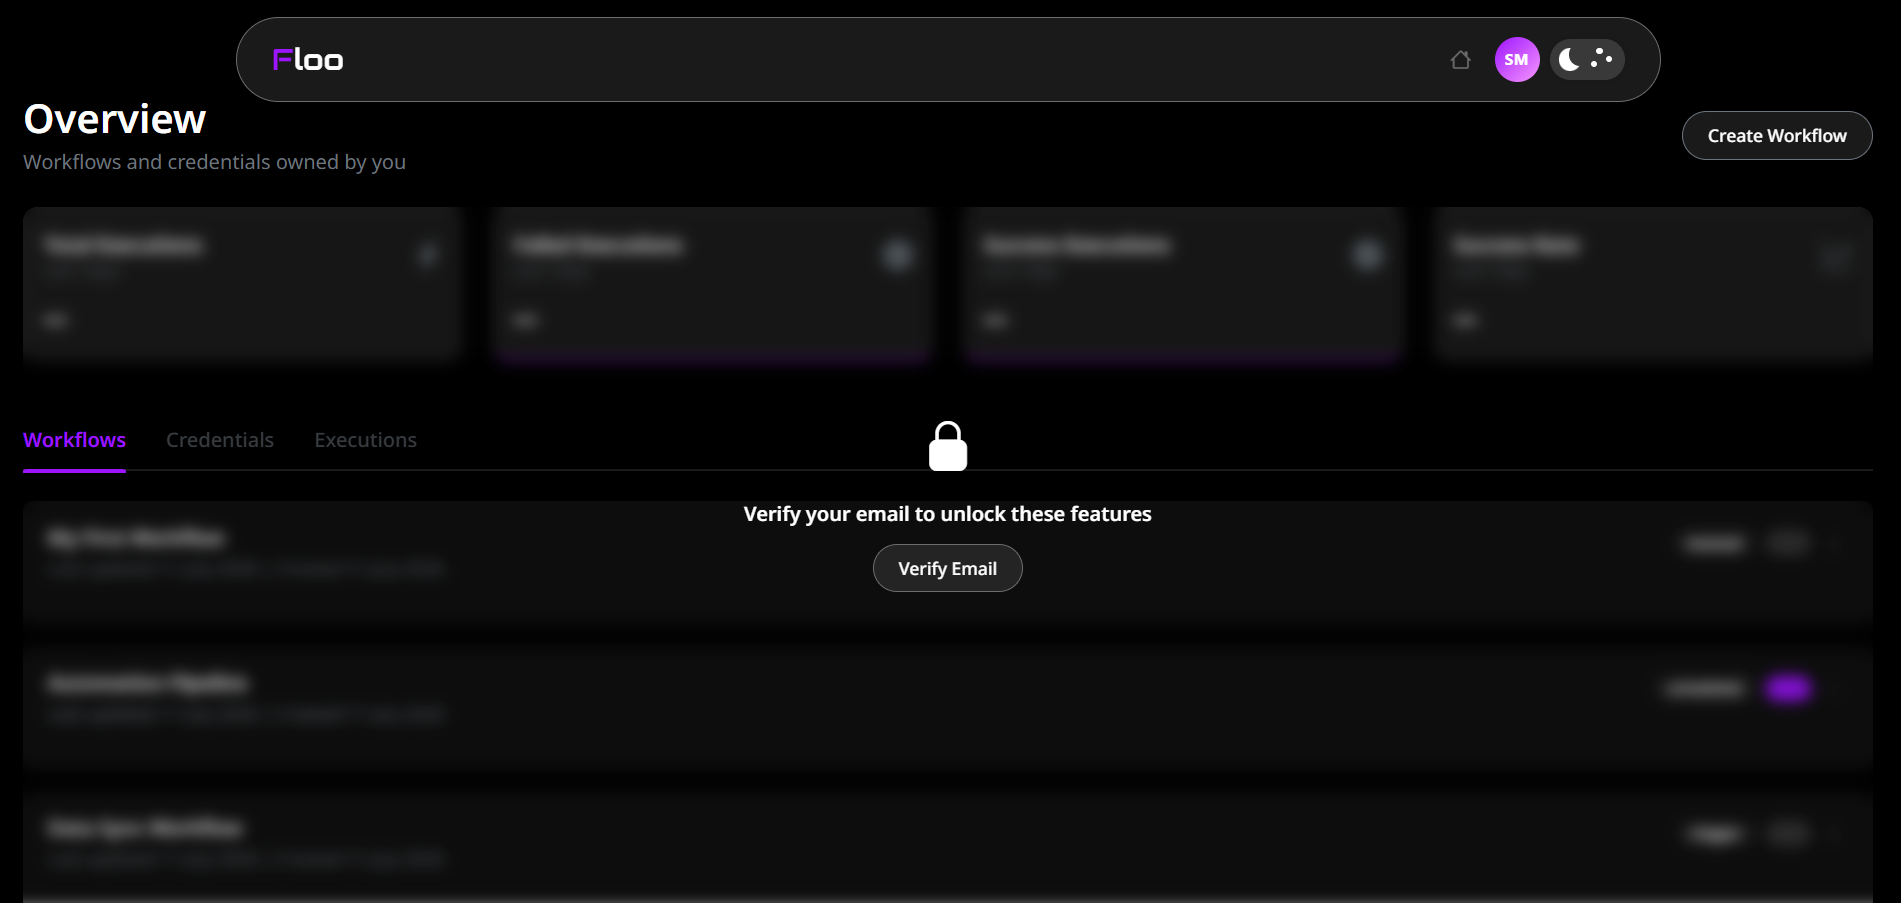
\includegraphics[width=\textwidth]{images/overview-page/disabled-overview.png}
    \caption{The Overview Page in restricted mode, showing blurred metrics, a disabled Workflows tab, and the email verification prompt.}
    \label{fig:overview-restricted-mode}
\end{figure}

\textbf{Purpose:} Prevents unauthorized access to workflow management features by placing the Overview page into a restricted mode whenever the user's email address is not verified, a state triggered after a user changes their email address and pending re-verification.

\vspace{0.2cm}
\noindent\textbf{Notes:}
\begin{itemize}
    \item The page remains accessible to preserve the application's layout and provide visual context, but all protected functionality is disabled; placeholder content and a verification prompt are shown instead of an empty page.
    \item The Create Workflow button is disabled and displays a tooltip indicating that email verification is required.
    \item The Metrics section remains visible but is covered by a blur overlay, preventing interaction with workflow statistics.
    \item The Credentials and Executions tabs are disabled and cannot be selected until the email is verified.
    \item The Workflows tab remains accessible but displays placeholder workflow cards instead of the user's actual workflows.
    \item A centered overlay containing a lock icon, an explanatory message, and a Verify Email button is displayed over the tab content.
    \item Selecting Verify Email resends the verification email, when necessary, and redirects the user to the email verification page to complete the process.
    \item Rather than hiding the Overview page completely, the system adopts a progressive restriction approach, letting users remain familiar with the interface while all operations requiring a verified identity stay securely disabled.
\end{itemize}